% !TeX root = ../main.tex
% !TeX root = ../main.tex
% Add the above to each chapter to make compiling the PDF easier in some editors.

\chapter{Scaling TUMLive}\label{chapter:introduction}

This chapter focuses on applying the concepts discussed in the previous sections to the architecture of TUMLive, discussing the development approach, results and challenges along the way. 

\section{Process, preparation, methods and environments}

The thesis spanned 5 months, from 15.05.2024 to \getSubmissionDate{}. The first weeks were spent familiarizing with the current system considering different approaches to scale its architecture and finding potential bottlenecks or issues. Following the initial analysis of the system, before being able to try scaling individual components, the original user and role system first needed to be updated together with new database models. After that, the most important components were gradually updated to be usable and manageable by each faculty. 
To develop and test the prototype of a distributed architecture for TUM-Live for this thesis, the following resources were used:
\begin{itemize}
    \item 3 \ac{VM}s with: 2 GB RAM, Intel(R) Xeon(R) CPU E5-2697A v4 @ 2.60GHz
    \item 1 \ac{VM} with: 20 GB RAM, AMD EPYC 7452 32-Core Processor
    \item 1 \ac{AWS} \ac{EKS} Cluster
    \item 1 selfhosted \ac{VM} with 32 GB RAM, AMD Ryzen 7 PRO 6850U @ 2.70GHz
\end{itemize}

After the target architecture had been deployed (on a smaller scale) using given resources, a set of performance tests and comparisons was made to find potential limits and breakpoints of each component. 
Additionally, in parallel to the development of the new architecture, a dedicated documentation has been created to facilitate the set up of GoCast for lecturers or new faculties which can be found at \href{https://tumlive-docs.pages.dev/}{tumlive-docs.pages.dev}. The documentation was created using Meta Opensource's Docusaurus. Static pages were deployed using Cloudflare.
All relevant source code for the thesis, new architecture, other mentioned prototypes and documentation can also be found at \href{https://github.com/carlobortolan/thesis}{github.com/carlobortolan/thesis}.

\section{Proposed System}

\subsection{Target System Architecture}

To distribute GoCast to different faculties, the subsystems and components responsible for processing and handling video data need to be distributed and hosted by each individual school. 
The main Tum-Live API instance however, will remain managed by the \ac{ITO} or TUM so that users have a single point of access (instead of having to switch instances when wanting to watch lectures of different faculties).
To achieve this, each faculty needs to host at least three components: the Runner / Worker component, the VoD service component and a Edge Server. 
Each school can then decide how many resources it wants to allocate to each service depending on their expected usage. The following minimum hardware requirements are set:

\begin{itemize}
    \item At least 1 VM as an Edge server. This server serves the videos to the users. Network throughput is important, so if a school serves many users, more instances are needed.
    \item At least 1 Worker or Runner VM. This server produces the stream, transcodes the VoD and much more. CPU performance is important here. On the same node, for every worker a VoD Service needs to be deployed to expose a simple HTTP interface that accepts file uploads and packages them to a HLS stream in a configured location. This stream may then be distributed by the Edge Server.
    \item Optionally, a school can add additional VMs for monitoring (grafana, prometheus, influx...) or for services such as the Voice Service for subtitling live streams and VoDs which requiring a NVIDIA CUDA equipped Server to transcribes streams using the Whisper LLM).
\end{itemize}

\begin{figure}[htpb]
    \centering
    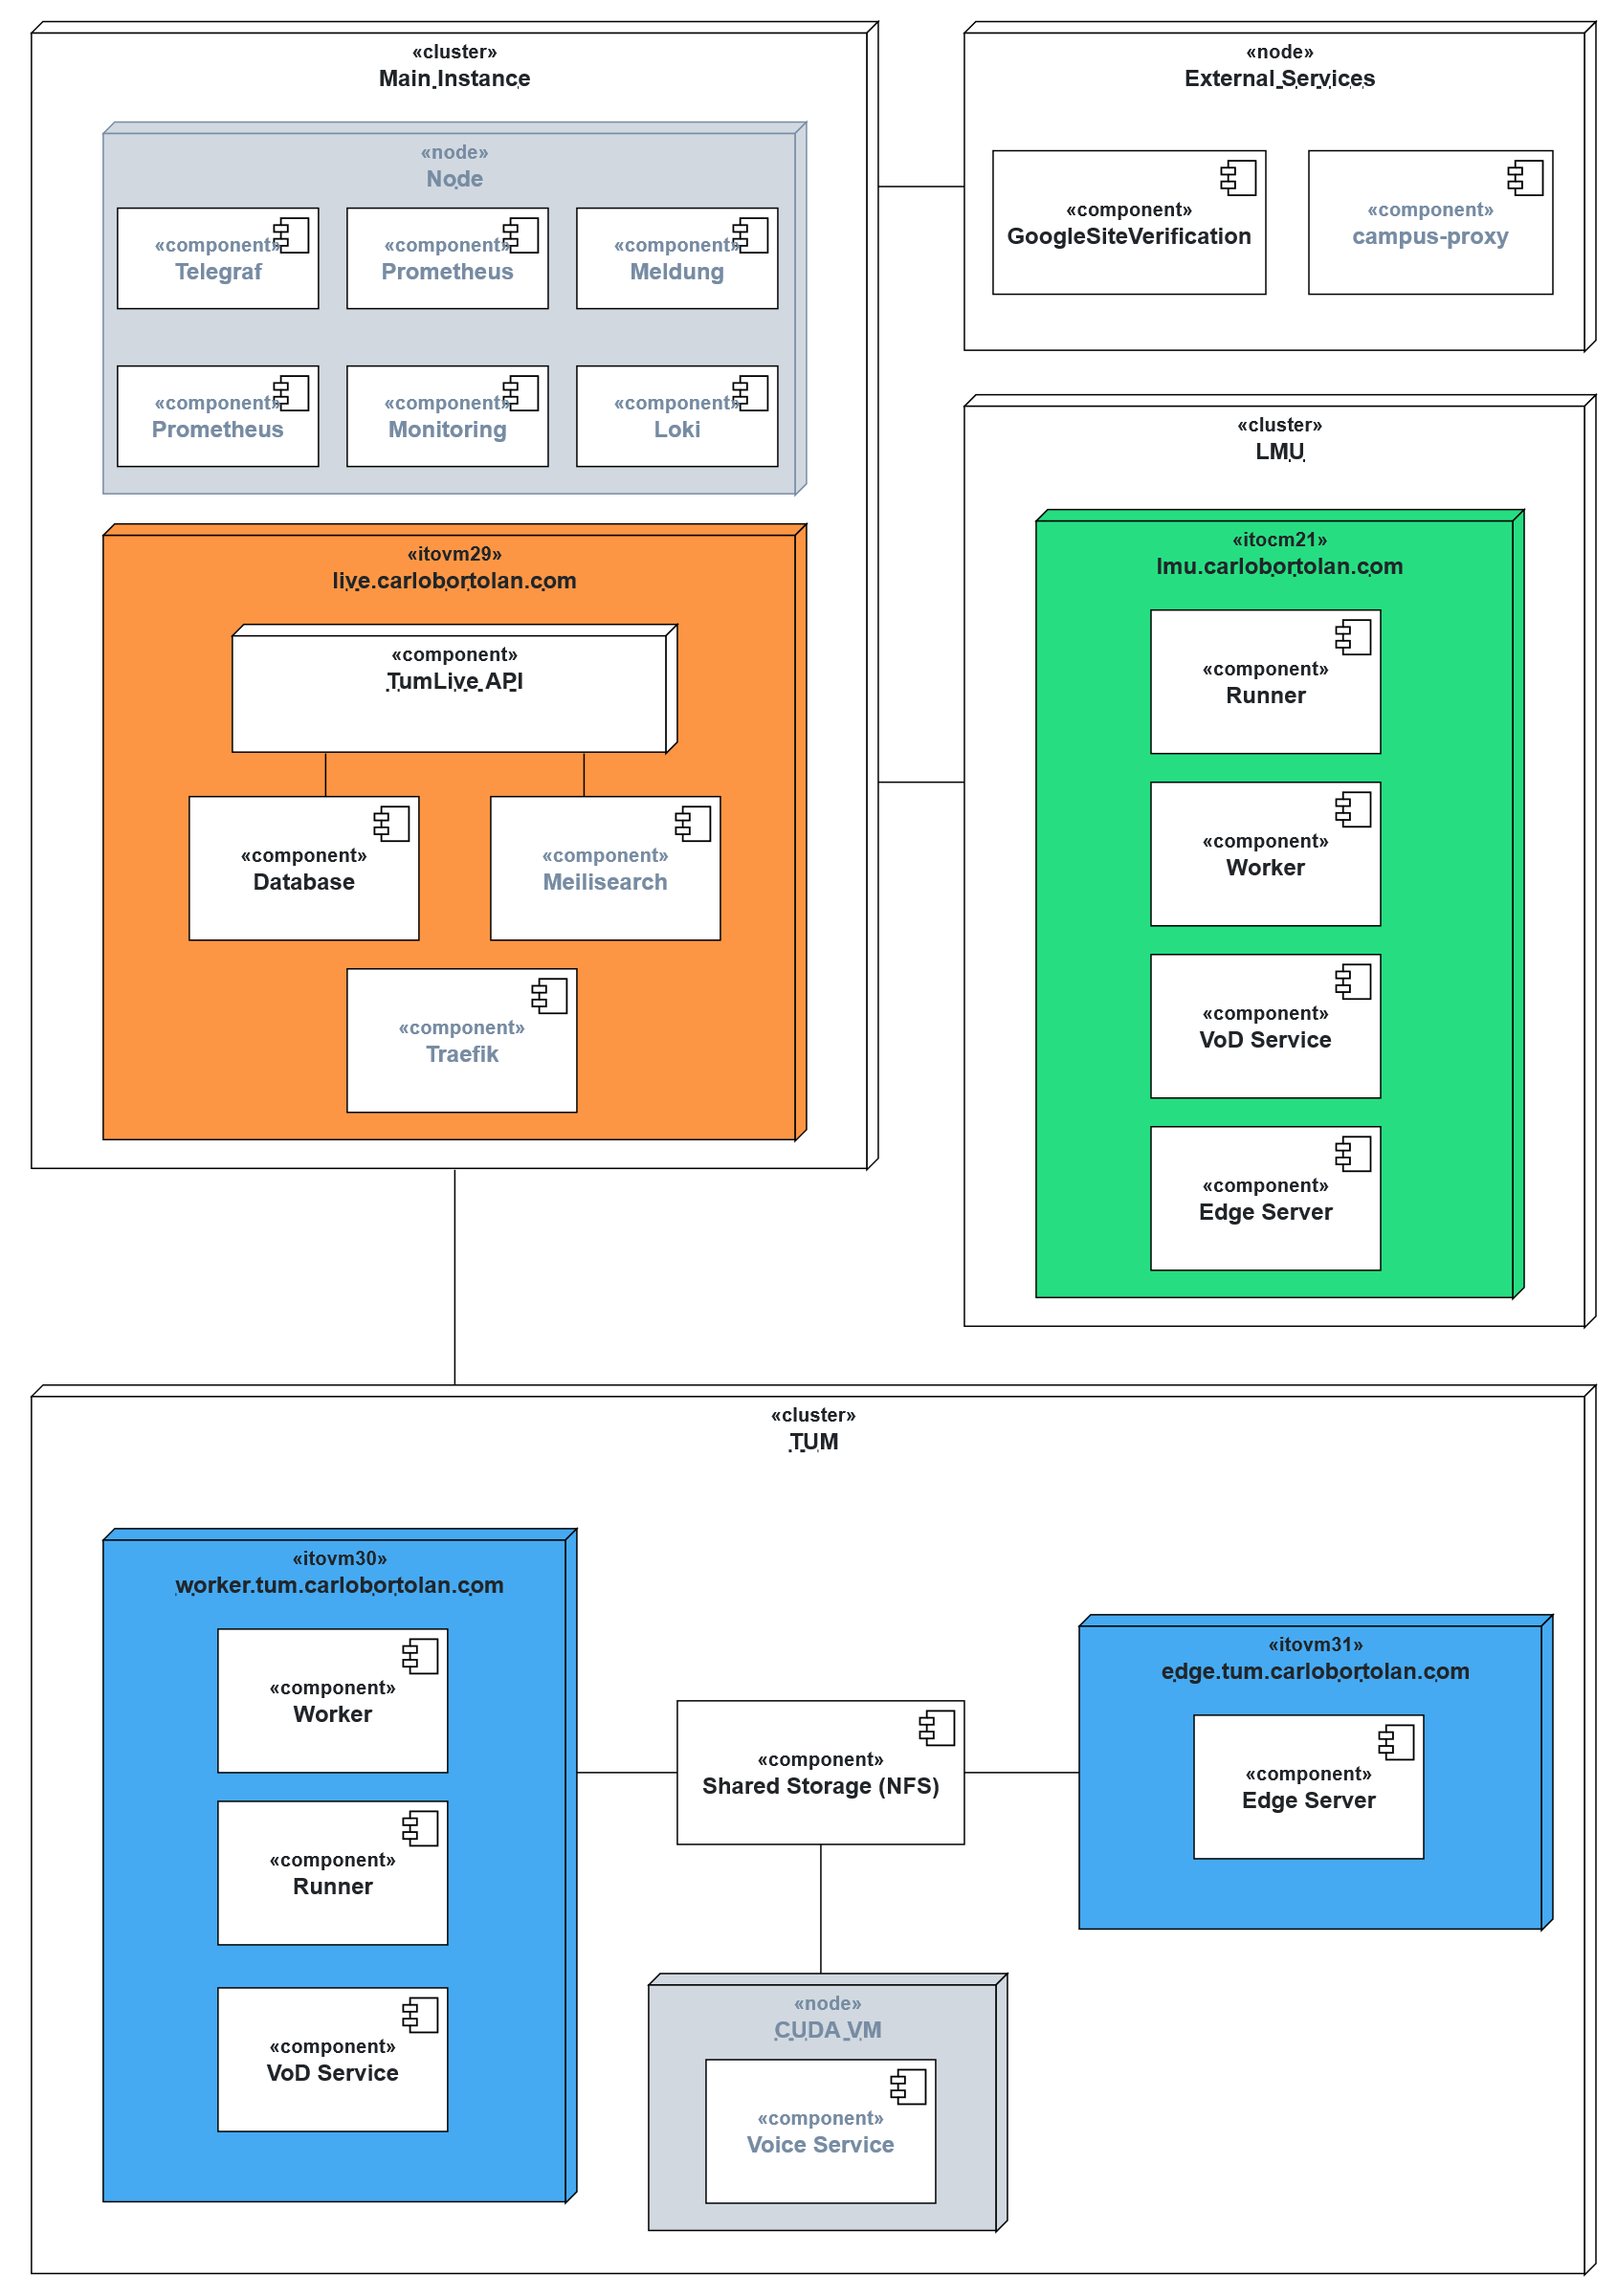
\includegraphics[width=\textwidth]{images/DeploymentDiagram.png}
    \caption[Target System Architecture]{Target Deployment Diagram of TUM-Live}\label{fig:system-architecture}
\end{figure}

\newpage


\section{Implementation Outline}

\subsection{Updating Architecture and Core API}

\subsection{Scaling Workers and Runners}

\subsection{Scaling Proxies and Other Services}

\subsection{Optimizing selected services}

\section{Introduction of Schools}

Initially, GoCast was used primarily by the former faculty of Informatics at TUM. However, with increasing demand, GoCast needs to be extended for university-wide lecture streaming. The solution to this are schools (not to be confused with TUMOnline's 'TUM School').

To start using GoCast for your department/school, you only need to deploy the TUM-Live Worker, VoD Service and TUM-Live Edge yourself. All other services are already provided by the GoCast network.

The idea is the following: To avoid one entity having to manage and process all streaming data for the entire university (or multiple universities), GoCast is distributed to multiple entities. Each entity (aka GoCast 'school') has so-called maintainers (users with the maintainer user role) that are allowed to manage the school's resources such as Workers/Runners, VoD Services, etc.

Maintainers also have some basic administrative functionality which is limited to their schools' scope (e.g., create, update and delete courses and streams only for those schools which are administered by that maintainer). For an overview of your administered schools, go to the "schools"-tab in the admin dashboard.
info

One maintainer can maintain multiple schools.
The following school-related actions are allowed by a maintainer of a school:

    Create, update or delete school

    Create new tokens for that school (required to add new resources)

    Manage school's resources

    Manage school's maintainers

TUMOnline School vs. GoCast School

TUMOnline has a strict hierarchical structure for its organizations (one school has multiple departments; one department has multiple chairs; one chair has multiple courses ...).
note

On a side node, TUMOnline has 7 schools, 29 departments and 487 chairs.

While GoCast is mainly used by the TUM, in principle it doesn't need to differentiate between organizational types that strictly. Organizations are only relevant when it comes to distributing the livestreams and recordings of a certain entity to that entity's resources (e.g., Workers/Runners and VoD Services). Hence, the introduction of GoCast's "schools" which represent an entity responsible for processing data. In practice, this is most of the time a TUMOnline school, however, in theory one could also create a GoCast "school" for a department, chair or smaller organization, depending on the specific situation.
Here's an example to illustrate this in a more detailled way:

    The TUMOnline "School of Management" (SOM) wants to start using GoCast. Hence, the SOM's IT team contacts the admins of GoCast who then create a new GoCast "school" of type TUM School and assign the SOM IT team as maintainers.

    The subordinated "Chair of Financial Management and Capital Markets" (FA), however, has its own data center and wants to host its lectures with its own resources. In this case, either one of the SOM maintainers or the RBG can create a new GoCast "school" of type Lehrstuhl and accordingly assign new maintainers from the FA-team. Now, the FA-team can connect their own resources from their data center with GoCast, independently of the SOM.

\section{Distributed Resources}

\subsection{Workers}
\subsection{Runners}
\subsection{Ingest Servers}
\subsection{Voice Service}

\section{Shared Resources}

